\newpage
	\flushright{\hyperref[index]{\color{black!65}{Ritorna all'indice}}}\flushleft
	\section{G} \label{sec:G}
		\subsection{GESTIONE DELLA CONFIGURAZIONE} \index{Gestione della configurazione} \label{gestioneconfigurazione}
		L'Analisi dei requisiti è un docmento collaborativo in cui ognuno ha la propria parte, non c'é confusione.
		
		\subsection{GESTIONE DEI CAMBIAMENTI} \index{Gestione dei cambiamenti} \label{gestionecambiamenti}
		Valuta la fattibilità tecnica e l'impatto sul progetto.
		[DETTO DAL PROF: L'Analisi dei requisiti non é un'attività libera da vincoli. Ogni cambiamento deve avere un resoconto (approfondiremo...).]
		
		\subsection{GESTIONE DEI REQUISITI}	\index{Gestione dei requisiti} \label{gestionerequisiti}
		Prevede l'identificazione e la \underline{\hyperref[classificazione]{classificazione}} dei \underline{\hyperref[requirements]{requisiti}}: identificatore unico, numerazione sequenziale basata sulla struttura del documento e le coppie (CATEGORIA, NUMERO). Avviene inoltre la \underline{\hyperref[gestionecambiamenti]{Gestione dei cambiamenti}} e la tracciabilità (Requisiti = parti della specifica = componenti del sistema).
		
		\subsection{GESTIONE DEI RISCHI} \index{Gestione dei rischi} \label{gestionerischi}
		Fa parte della \underline{\hyperref[gestioneprogetto]{Gestione di progetto}}. Prevede:
			\begin{itemize}
				\item Identificazione dei rischi nel progetto, nel prodotto e nel mercato;
				\item Analisi della probabilità di occorrenza e conseguenze possibili;
				\item Pianificazione, ovvero come evitare i rischi e mitigarne gli effetti;
				\item Controllo, ovvero attenzione continua tramite rilevazione di indicatori e raffinamento delle strategie;
			\end{itemize}
		\begin{figure}[H]
			\centering
			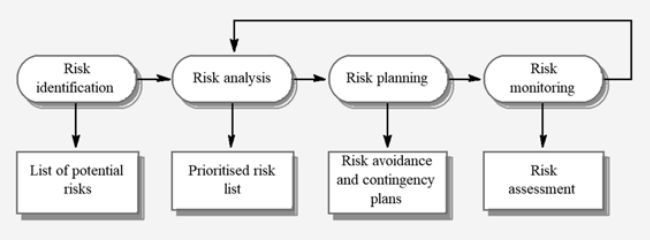
\includegraphics[width=0.8\textwidth]{img/rischi}		
			\caption{Schema della gestione dei rischi.}
		\end{figure} 
		I principali \textit{fattori di successo} sono il coinvolgimento del cliente, supporto della direzione esecutiva, definizione chiara dei requisiti, pianificazione corretta, aspettative realistiche e personale competente. Mentre i primi \textit{fattori di fallimento} sono requisiti incompleti, mancato coinvolgimento del cliente, mancanza di risorse, aspettative non realistiche e mancanza di supporto  esecutivo.
		
		
		\subsection{GESTIONE DI PROGETTO} \index{Gestione di progetto} \label{gestioneprogetto}	%V.I.
		La gestione di progetto prevede:
			\begin{itemize}
				\item l'istanziazione di processi nel progetto secondo: \underline{\hyperref[standard]{standard di processo}} che istanziano processi aziendali che istanziano processi di progetto;
				\item la stima di costi e risorse necessarie (fattori di influenza per le stime: dimensione del progetto, esperienza del dominio, familiarità con le tecnologie, produttività dell'ambiente di lavoro, \underline{\hyperref[qualita]{qualità}} attesa) tramite \underline{\hyperref[cocomo]{CoCoMo}};
				\item \underline{\hyperref[pianificazione]{Pianificazione}} (partendo dall'obiettivo, non dall'inizio) di attività con conseguente assegnamento alle varie persone; 
				\item il controllo delle attività e la verifica dei risultati;
			\end{itemize}
		In questo contesto ogni persona assume un certo \underline{\hyperref[ruoli]{ruolo}} e ad ogni ruolo viene assegnata un'attività (notare che spesso molte risorse sono impegnate su più progetti). La gestione di progetto prevede anche la  \underline{\hyperref[gestionequalita]{Gestione di Qualità}} e un \underline{\hyperref[piano]{Piano di progetto}}.
		
		\subsection{GESTIONE DI QUALITÀ}  \index{Gestione di qualità} \label{gestionequalita}
		È una funzione aziendale e con precisione, la funzione di più recente introduzione. La \underline{\hyperref[qualita]{qualità}} riguarda qui sia i prodotti che i processi e interessa sia committente che la direzione aziendale. La garanzia di qualità produce confidenza, richiede l'applicazione rigorosa dei processi adottati e la loro \underline{\hyperref[manutenzione]{manutenzione}} migliorativa (ciclo di \underline{\hyperref[pdca]{PDCA}}).
	
	
